\documentclass[aspectratio=169,12pt]{beamer}

\usepackage[fontset=none]{ctex}
\usepackage{fontspec}
\setmainfont{Noto Sans CJK SC}
\setsansfont{Noto Sans CJK SC}
\setCJKmainfont{Noto Sans CJK SC}
\setCJKsansfont{Noto Sans CJK SC}
\setCJKmonofont{Noto Sans CJK SC}

\usepackage{tikz}
\usepackage{pgfplots}
\pgfplotsset{compat=1.18}

\definecolor{mx}{HTML}{CC3E22}
\definecolor{mxdark}{HTML}{8C2F1B}
\definecolor{mxsoft}{HTML}{E7B2A6}
\definecolor{ink}{HTML}{262626}
\definecolor{muted}{HTML}{6B6562}
\definecolor{paper}{HTML}{FBF8F6}
\definecolor{band}{HTML}{F6E7E2}

\setbeamercolor{normal text}{fg=ink,bg=white}
\setbeamercolor{structure}{fg=mx}
\setbeamercolor{frametitle}{fg=white,bg=mx}
\setbeamercolor{title}{fg=ink}
\setbeamercolor{subtitle}{fg=muted}
\setbeamercolor{item}{fg=mx}
\setbeamercolor{footer}{fg=muted,bg=paper}
\setbeamerfont{frametitle}{size=\Large,series=\bfseries}
\setbeamerfont{title}{size=\LARGE,series=\bfseries}
\setbeamerfont{footer}{size=\scriptsize}
\setbeamertemplate{navigation symbols}{}
\setbeamertemplate{itemize item}{\small\raise1pt\hbox{\textcolor{mx}{\rule{0.45em}{0.45em}}}}
\setbeamertemplate{itemize subitem}{\scriptsize\textcolor{mxsoft}{\rule{0.38em}{0.38em}}}

\setbeamertemplate{frametitle}{%
  \nointerlineskip
  \begin{beamercolorbox}[wd=\paperwidth,ht=2.55em,dp=0.7em,leftskip=1.15em]{frametitle}%
    \usebeamerfont{frametitle}\insertframetitle
  \end{beamercolorbox}%
}

\setbeamertemplate{footline}{%
  \leavevmode
  \hbox{%
    \begin{beamercolorbox}[wd=\paperwidth,ht=2.5ex,dp=1.1ex,leftskip=1.15em,rightskip=1.15em]{footer}%
      \usebeamerfont{footer}闽信保险有限公司\hfill 演示口径，仅供看版式\hfill \insertframenumber\,/\,\inserttotalframenumber
    \end{beamercolorbox}%
  }%
}

\title{闽信保险有限公司}
\subtitle{2026年度业务汇报}
\author{汇报人：演示}
\date{2026.3}
\pgfplotsset{
  tick label style={font=\small,color=ink},
  label style={font=\small,color=muted},
  legend style={font=\small,draw=none,fill=none},
  every axis plot/.append style={line width=1.1pt},
}

\begin{document}

\begin{frame}[plain]
  \begin{tikzpicture}[remember picture,overlay]
    \fill[mx] (current page.north west) rectangle ([yshift=-0.42cm]current page.north east);
    \fill[band] ([yshift=1.55cm]current page.south west) rectangle (current page.south east);
  \end{tikzpicture}
  \vspace{1.35cm}
  {\color{mx}\bfseries\footnotesize 演示稿\quad Beamer / XeLaTeX}\\[0.7em]
  {\usebeamerfont{title}\usebeamercolor[fg]{title}闽信保险有限公司}\\[0.35em]
  {\Large 2026年度业务汇报}\\[1.1em]
  {\color{muted}汇报人：演示\quad 时间：2026.3}\\[1.6em]
  {\color{ink}三张图都是演示数据：柱状图、饼图、折线图。}
\end{frame}

\begin{frame}{汇报目录}
  \begin{columns}[T,onlytextwidth]
    \begin{column}{0.32\textwidth}
      \textcolor{mx}{\bfseries 01}\\[0.3em]
      {\large 企业概况}\\[0.45em]
      {\small\color{muted}服务定位、市场和主要险种。}
    \end{column}
    \begin{column}{0.32\textwidth}
      \textcolor{mx}{\bfseries 02}\\[0.3em]
      {\large 三张图}\\[0.45em]
      {\small\color{muted}保费柱状图、险种饼图、赔付率折线。}
    \end{column}
    \begin{column}{0.32\textwidth}
      \textcolor{mx}{\bfseries 03}\\[0.3em]
      {\large 怎么读}\\[0.45em]
      {\small\color{muted}数字只为看版式，不代表经营结果。}
    \end{column}
  \end{columns}
  \vspace{1.3em}
  \begin{itemize}
    \item 幻灯片由 Beamer 直接排版，字体嵌在 PDF 里。
    \item 图用 TikZ 和 pgfplots 画，是矢量图，不是贴上去的图片。
  \end{itemize}
\end{frame}

\begin{frame}{企业概况}
  \begin{columns}[T,onlytextwidth]
    \begin{column}{0.32\textwidth}
      {\color{mx}\bfseries 公司定位}\\[0.4em]
      立足香港的专业财产险服务商，为企业客户提供风险保障。
    \end{column}
    \begin{column}{0.32\textwidth}
      {\color{mx}\bfseries 业务范围}\\[0.4em]
      以企业财产险、责任险、工程险为主，按行业场景设计方案。
    \end{column}
    \begin{column}{0.32\textwidth}
      {\color{mx}\bfseries 这页之后}\\[0.4em]
      用三张图看规模、结构和赔付。坐标和比例都是演示口径。
    \end{column}
  \end{columns}
\end{frame}

\begin{frame}{保费收入：柱状图}
  \vspace{-0.4em}
  {\small\color{muted}演示数据，单位：亿元。柱顶数字是该年保费。}
  \vspace{0.2em}
  \begin{center}
  \begin{tikzpicture}
    \begin{axis}[
      ybar,
      bar width=18pt,
      width=0.92\textwidth,
      height=0.62\textheight,
      ymin=0, ymax=30,
      ylabel={亿元},
      symbolic x coords={2023,2024,2025},
      xtick=data,
      axis line style={draw=muted},
      tick style={draw=muted},
      ymajorgrids=true,
      grid style={draw=band},
      nodes near coords,
      every node near coord/.append style={font=\small,color=mxdark},
      enlarge x limits=0.35,
    ]
      \addplot[fill=mx,draw=none] coordinates {(2023,18.6) (2024,21.4) (2025,24.1)};
    \end{axis}
  \end{tikzpicture}
  \end{center}
\end{frame}

\begin{frame}{险种结构：饼图}
  \vspace{-0.3em}
  {\small\color{muted}演示数据。三块合计 100\%。}
  \vspace{0.6em}
  \begin{columns}[c,onlytextwidth]
    \begin{column}{0.52\textwidth}
      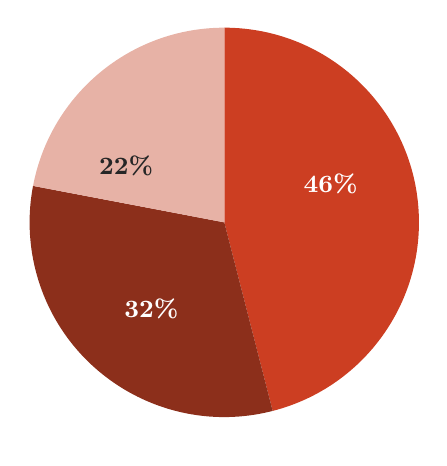
\begin{tikzpicture}[scale=1.15]
        % 46% = 165.6°, 32% = 115.2°, 22% = 79.2°. Start at 90°.
        \fill[mx] (0,0) -- (90:2.15) arc (90:-75.6:2.15) -- cycle;
        \fill[mxdark] (0,0) -- (-75.6:2.15) arc (-75.6:-190.8:2.15) -- cycle;
        \fill[mxsoft] (0,0) -- (-190.8:2.15) arc (-190.8:-270:2.15) -- cycle;
        \node[font=\small\bfseries,text=white] at (20:1.25) {46\%};
        \node[font=\small\bfseries,text=white] at (-130:1.25) {32\%};
        \node[font=\small\bfseries,text=ink] at (150:1.25) {22\%};
      \end{tikzpicture}
    \end{column}
    \begin{column}{0.42\textwidth}
      \textcolor{mx}{\rule{0.7em}{0.7em}}\quad 企业财产险\quad 46\%\\[0.7em]
      \textcolor{mxdark}{\rule{0.7em}{0.7em}}\quad 责任险\quad 32\%\\[0.7em]
      \textcolor{mxsoft}{\rule{0.7em}{0.7em}}\quad 工程险\quad 22\%\\[1.1em]
      {\small\color{muted}财产险是基本盘。责任险和工程险用来看结构，不代表真实承保占比。}
    \end{column}
  \end{columns}
\end{frame}

\begin{frame}{赔付率：折线图}
  \vspace{-0.4em}
  {\small\color{muted}演示数据，单位：\%。折线逐年下降，只为展示走势。}
  \vspace{0.2em}
  \begin{center}
  \begin{tikzpicture}
    \begin{axis}[
      width=0.92\textwidth,
      height=0.62\textheight,
      ymin=40, ymax=70,
      ylabel={\%},
      symbolic x coords={2023,2024,2025},
      xtick=data,
      axis line style={draw=muted},
      tick style={draw=muted},
      ymajorgrids=true,
      grid style={draw=band},
      enlarge x limits=0.25,
    ]
      \addplot[color=mx,mark=*,mark size=2.4pt,mark options={fill=mx,draw=mx}] coordinates {(2023,58) (2024,54) (2025,49)};
      \node[font=\small,text=mxdark,anchor=south] at (axis cs:2023,58) {58};
      \node[font=\small,text=mxdark,anchor=south] at (axis cs:2024,54) {54};
      \node[font=\small,text=mxdark,anchor=south west] at (axis cs:2025,49) {49};
    \end{axis}
  \end{tikzpicture}
  \end{center}
\end{frame}

\begin{frame}[plain]
  \begin{tikzpicture}[remember picture,overlay]
    \fill[mx] (current page.north west) rectangle ([yshift=-0.42cm]current page.north east);
    \fill[band] ([yshift=1.55cm]current page.south west) rectangle (current page.south east);
  \end{tikzpicture}
  \vspace{2.2cm}
  {\usebeamerfont{title}感谢聆听}\\[0.6em]
  {\color{muted}闽信与您，共筑安全未来}\\[1.2em]
  {\small\color{ink}这页四个字来自同一套 Noto Sans CJK，不会再出现缺字换字体。}
\end{frame}

\end{document}
